\section{Additional 20,000-Subscription Handoff Diagnostics}
\label{app:cloud-timing}
The deployment setup and aggregate results appear in the main paper. The
following paired plot retains the within-run timing detail.
\begin{figure}[!htbp]
  \centering
  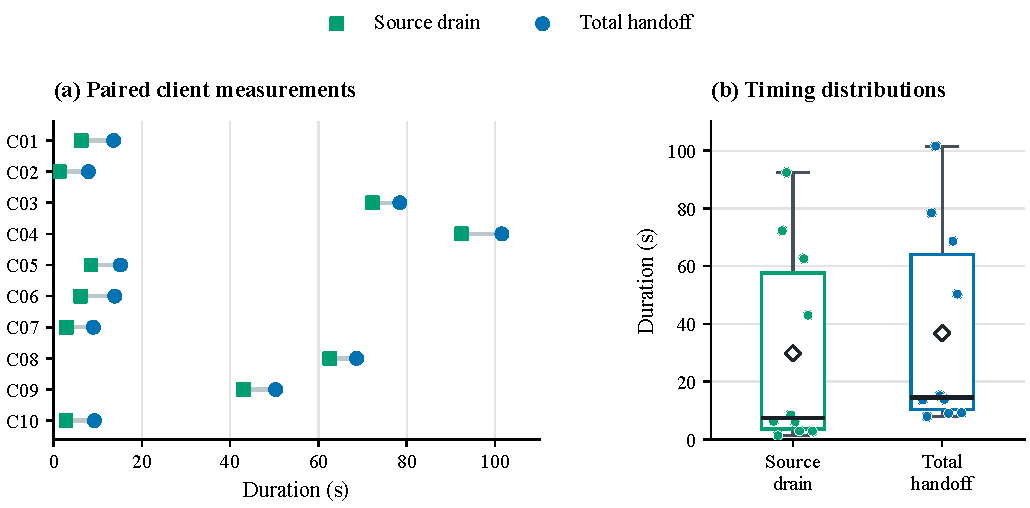
\includegraphics[width=\textwidth]{figures/mumbai-handoff-boxplots.pdf}
  \caption{Measured Oracle Cloud cluster migration timing. Left: paired source-drain and
  total-handoff durations for each of the ten client migrations. Right:
  quartile boxes with median lines, mean diamonds, and all ten observations;
  whiskers extend to observations within 1.5 interquartile ranges. These are
  ten migrations in one cluster run, not ten independent cluster trials.}
  \Description{Paired duration markers and box plots show source drain and
  total handoff for ten clients. Longer handoffs coincide with longer source
  drain waits. Drain is a component of
  total handoff, not an additional duration.}
  \label{fig:mumbai-handoff-distributions}
\end{figure}


Figure~\ref{fig:mumbai-handoff-distributions} retains the pairing that a
summary median cannot show. For client $u$, the interval between its two
markers is $T^{\mathrm{handoff}}_u-T^{\mathrm{drain}}_u$, the measured non-drain remainder of
the handoff; it is not an estimate of network latency alone. The box extends
from the sample's first to third quartile, so the interquartile range describes
the central half of the timings. All points, including the long-duration
observations, remain visible. Longer handoffs coincide with longer source
drains, consistent with the receipt-gated mechanism waiting for outstanding
work. These are within-run timing distributions; their scope is the observed
deployment, without a between-deployment confidence interval.

An independent collector retained 31 observations of each of the ten pods
over approximately 2,422 seconds. All pods remained Ready, with unchanged
pod, image, and process identities and no restart increase. These observations
establish operational continuity over this observation period. Long-term
availability is outside the measurement window.
